% Cover 3: "Terminal Green" — Black bg, matrix-green data streams, quant/hacker aesthetic
\documentclass[tikz,border=0mm]{standalone}
\usepackage{tikz}
\usetikzlibrary{calc,decorations.markings}
\usepackage{xcolor}
\usepackage[T1]{fontenc}

\definecolor{termblack}{RGB}{8,12,8}
\definecolor{termgreen}{RGB}{0,200,80}
\definecolor{termgreenbright}{RGB}{80,255,140}
\definecolor{termgreendim}{RGB}{0,100,40}
\definecolor{termgreenpale}{RGB}{180,255,200}
\definecolor{amber}{RGB}{255,176,0}
\definecolor{amberdim}{RGB}{160,100,0}

\begin{document}
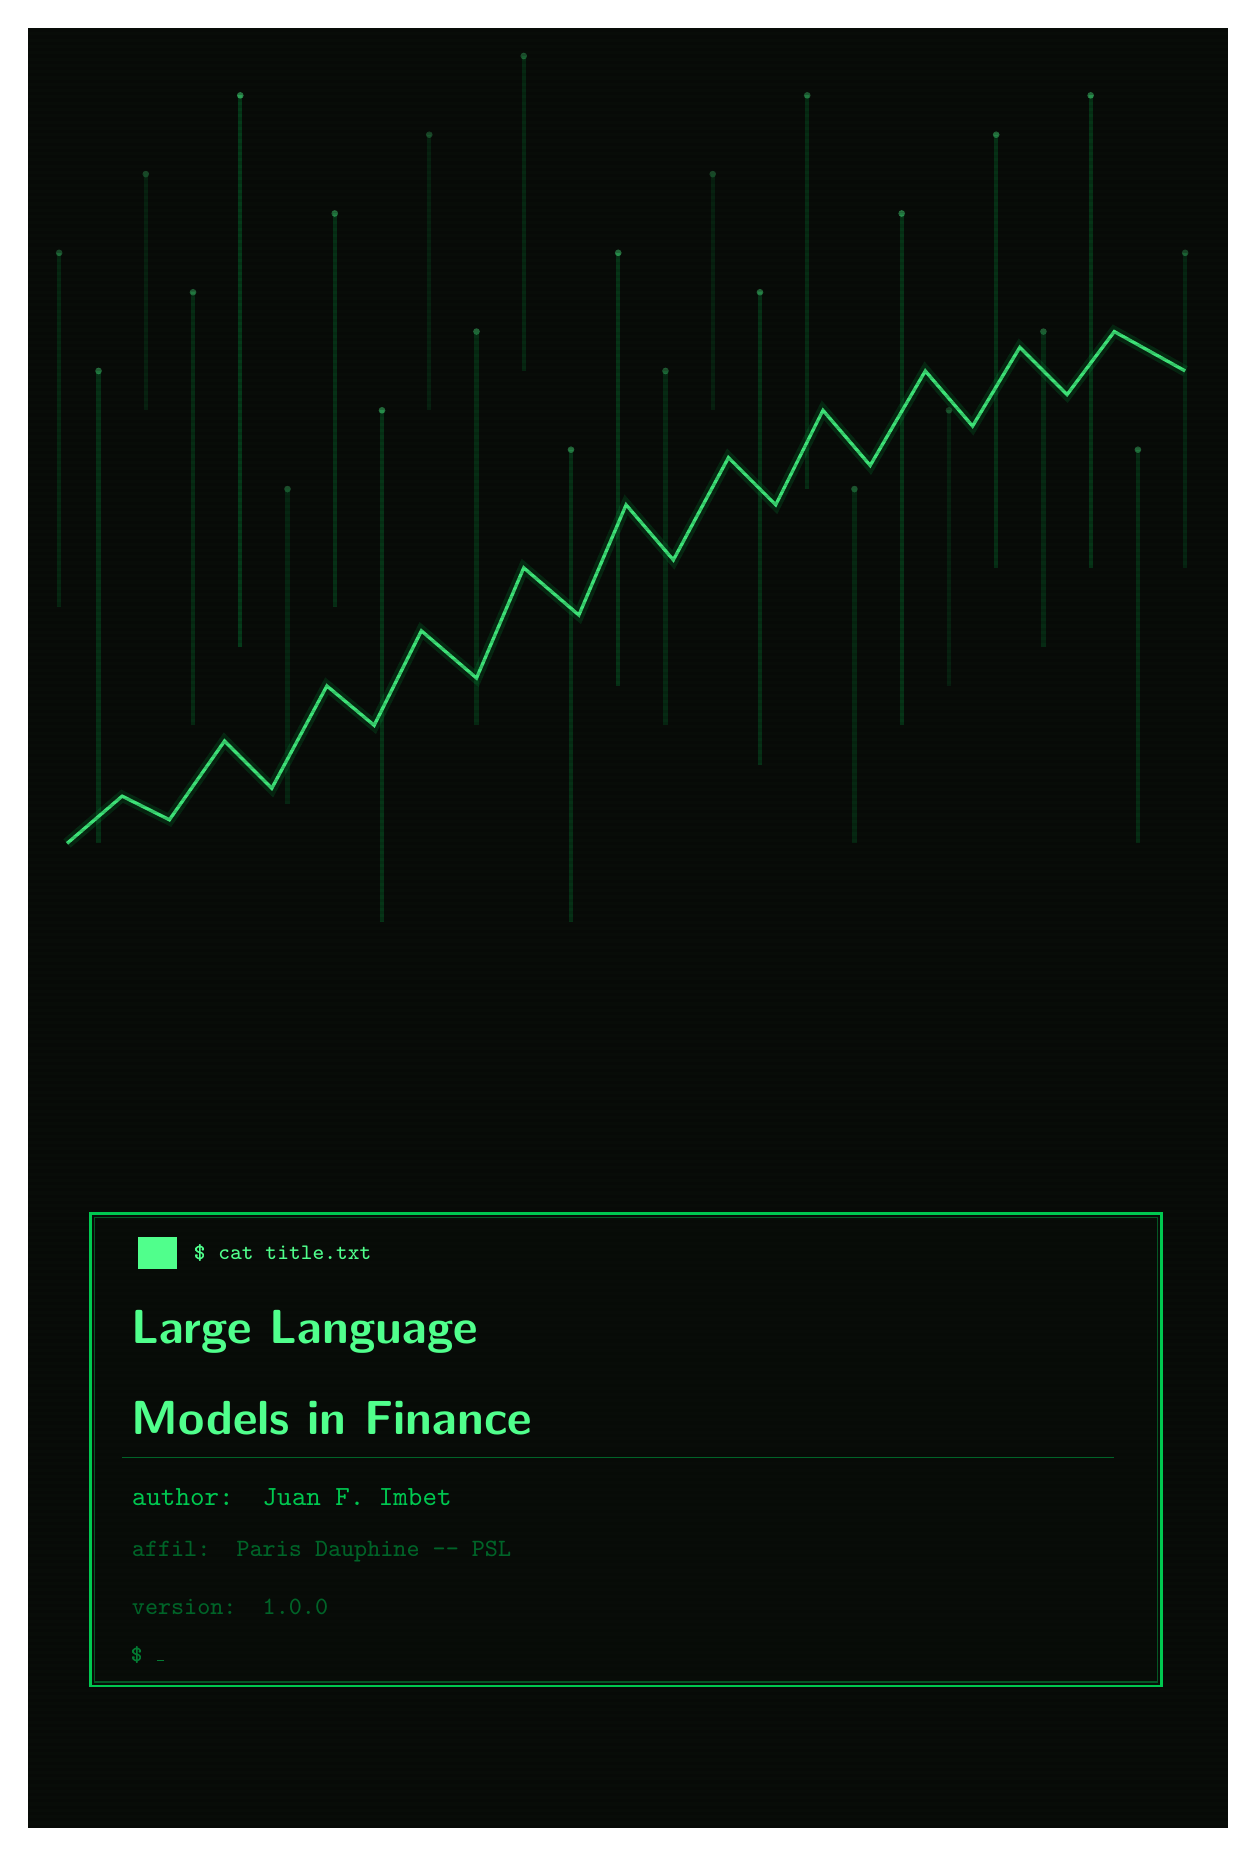
\begin{tikzpicture}
  % --- background ---
  \fill[termblack] (0,0) rectangle (15.24,22.86);

  % --- matrix rain columns (vertical streams of characters/bars) ---
  % Simulate with varying-opacity vertical lines of different lengths
  \foreach \x/\top/\len/\op in {
    0.4/20.0/4.5/0.15,  0.9/18.5/6.0/0.20,  1.5/21.0/3.0/0.12,
    2.1/19.5/5.5/0.18,  2.7/22.0/7.0/0.25,  3.3/17.0/4.0/0.14,
    3.9/20.5/5.0/0.20,  4.5/18.0/6.5/0.22,  5.1/21.5/3.5/0.12,
    5.7/19.0/5.0/0.18,  6.3/22.5/4.0/0.15,  6.9/17.5/6.0/0.20,
    7.5/20.0/5.5/0.22,  8.1/18.5/4.5/0.16,  8.7/21.0/3.0/0.12,
    9.3/19.5/6.0/0.20,  9.9/22.0/5.0/0.18, 10.5/17.0/4.5/0.15,
    11.1/20.5/6.5/0.22, 11.7/18.0/3.5/0.12, 12.3/21.5/5.5/0.20,
    12.9/19.0/4.0/0.16, 13.5/22.0/6.0/0.22, 14.1/17.5/5.0/0.18,
    14.7/20.0/4.0/0.14
  }{
    \pgfmathsetmacro{\bot}{\top-\len}
    \draw[termgreen,opacity=\op,line width=1.5pt] (\x,\bot) -- (\x,\top);
    % bright leading dot
    \fill[termgreenbright,opacity=\op*2.0] (\x,\top) circle (1.2pt);
  }

  % --- time-series line (financial price path) ---
  % Bright green line across the middle zone
  \draw[termgreenbright,line width=1.2pt,opacity=0.9]
    (0.5,12.5) -- (1.2,13.1) -- (1.8,12.8) -- (2.5,13.8) -- (3.1,13.2)
    -- (3.8,14.5) -- (4.4,14.0) -- (5.0,15.2) -- (5.7,14.6) -- (6.3,16.0)
    -- (7.0,15.4) -- (7.6,16.8) -- (8.2,16.1) -- (8.9,17.4) -- (9.5,16.8)
    -- (10.1,18.0) -- (10.7,17.3) -- (11.4,18.5) -- (12.0,17.8)
    -- (12.6,18.8) -- (13.2,18.2) -- (13.8,19.0) -- (14.7,18.5);
  % glow effect (thicker, low opacity)
  \draw[termgreen,line width=4pt,opacity=0.15]
    (0.5,12.5) -- (1.2,13.1) -- (1.8,12.8) -- (2.5,13.8) -- (3.1,13.2)
    -- (3.8,14.5) -- (4.4,14.0) -- (5.0,15.2) -- (5.7,14.6) -- (6.3,16.0)
    -- (7.0,15.4) -- (7.6,16.8) -- (8.2,16.1) -- (8.9,17.4) -- (9.5,16.8)
    -- (10.1,18.0) -- (10.7,17.3) -- (11.4,18.5) -- (12.0,17.8)
    -- (12.6,18.8) -- (13.2,18.2) -- (13.8,19.0) -- (14.7,18.5);

  % --- horizontal scan lines (CRT effect) ---
  \foreach \y in {0,0.08,...,22.86}{
    \fill[black,opacity=0.12] (0,\y) rectangle (15.24,\y+0.04);
  }

  % --- title box ---
  \fill[termblack,opacity=0.85] (0.8,1.8) rectangle (14.4,7.8);
  \draw[termgreen,line width=1.0pt] (0.8,1.8) rectangle (14.4,7.8);
  \draw[termgreen,line width=0.4pt,opacity=0.4] (0.85,1.85) rectangle (14.35,7.75);

  % blinking cursor accent
  \fill[termgreenbright] (1.4,7.1) rectangle (1.9,7.5);

  \node[anchor=west,text=termgreenbright,font=\fontsize{8}{10}\selectfont\ttfamily]
    at (2.0,7.3) {\$ cat title.txt};

  \node[anchor=west,text=termgreenbright,font=\fontsize{18}{20}\selectfont\sffamily\bfseries]
    at (1.2,6.3) {Large Language};
  \node[anchor=west,text=termgreenbright,font=\fontsize{18}{20}\selectfont\sffamily\bfseries]
    at (1.2,5.2) {Models in Finance};

  \draw[termgreendim,line width=0.5pt] (1.2,4.7) -- (13.8,4.7);

  \node[anchor=west,text=termgreen,font=\fontsize{10}{12}\selectfont\ttfamily]
    at (1.2,4.2) {author:  Juan F. Imbet};
  \node[anchor=west,text=termgreendim,font=\fontsize{9}{11}\selectfont\ttfamily]
    at (1.2,3.5) {affil:   Paris Dauphine -- PSL};
  \node[anchor=west,text=termgreendim,font=\fontsize{9}{11}\selectfont\ttfamily]
    at (1.2,2.8) {version: 1.0.0};
  \node[anchor=west,text=termgreen,font=\fontsize{8}{10}\selectfont\ttfamily,opacity=0.6]
    at (1.2,2.2) {\$ \textunderscore};

\end{tikzpicture}
\end{document}
